\Chapter{Encryptie - Applicaties}

\emph{Citations needed}

Sinds het begin der tijden is er een nood geweest aan manieren om berichten versleuteld te verzenden tussen twee partijen. Voorbeelden van enkele klassieke encryptiemethoden zijn het Atbashcijfer~\cite{atbash} (Babyloni"e, 600 v. Chr.), het Caesarcijfer~\cite{caesar} (56 n. Chr.) en het dubbele transpositie cijfer~\cite{double-transp} (oa. gebruikt door weerstandsgroepen in WO II). E'en eigenschap die al deze methodes met elkaar gemeen hebben, is het gebruik van een op voorhand afgesproken sleutel. Dit principe, dat ook door vele moderne encryptiemethodes (zoals bv. 3DES~\cite{3DES} en AES~\cite{AES}) gebruikt wordt, noemt men symetrische versleuteling.

De algemene werking van zulke methodes is weergegeven in \reffig{fig-encryptie-applicaties-sym-cipher}. Alice zendt een bericht $m$ naar Bob door het te versleutelen, met een door hen beiden gekende sleutel $k$, die op zijn beurt met diezelfde sleutel het bericht ontcijfert. Indien Eve de vooraf afgesproken sleutel kent, kan zij uiteraard alle communicatie tussen Alice en Bob ontcijferen. Er is dus nood aan een manier om veilig een sleutel $k$ te kunnen afspreken tussen twee partijen. Deze sleutel kan dan vervolgens bijvoorbeeld gebruikt worden in een symmetrisch sleutel algoritme.

\vspace{\textfloatsep}
\begin{minipage}{\linewidth}
    \begin{center}
    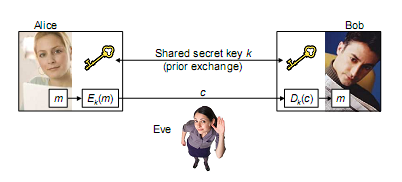
\includegraphics[width=7cm]{symmetric-cipher-model}
    \figcaption{Algemene structuur van een symmetrische versleutelingsmethode}\label{fig-encryptie-applicaties-sym-cipher}
    \end{center}
    \end{minipage}
\vspace{\textfloatsep}

Een oplossing voor dit probleem was niet gekend tot en met 1976, toen Diffie en Hellman hun algoritme voor sleutel uitwisseling~\cite{diffie-hellman} publiceerden. Hun algoritme laat twee partijen toe een geheime sleutel over een onbeveiligd kanaal af te spreken. Deze ontdekking plaveide de weg voor talrijke publieke sleutel methodes (oftewel asymmetrische sleutel methodes), waarvan de werking wordt getoond in \reffig{fig-encryptie-applicaties-asym-cipher}.

\vspace{\textfloatsep}
\begin{minipage}{\linewidth}
    \begin{center}
    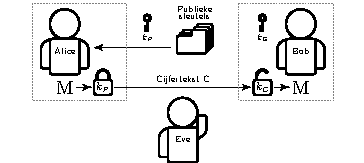
\includegraphics[width=7cm]{asymmetric-cipher-model}
    \figcaption{Algemene structuur van een asymmetrische versleutelingsmethode}\label{fig-encryptie-applicaties-asym-cipher}
    \end{center}
    \end{minipage}
\vspace{\textfloatsep}